\chapter{Planificación y requisitos}\label{cap.requisitos}
\section{Introducción}
Para unos resultados satisfactorios, es crucial plantear las labores que se han de realizar y analizar los requisitos que ha de reunir el simulador, así como distribuir las tareas en el tiempo disponible.

Por ello, el primer paso que se ha de realizar es el análisis de \textit{QuaDRiGa} para identificar qué características han de ser implementadas para complementarlo.

Además, resulta igual de importante distribuir las tareas en las 300 horas de las que se dispone, así como identificar los recursos software, hardware y humanos con los que se cuenta para la elaboración del proyecto.

\section{Requisitos}
Como se introducía en el anterior capítulo, se han de tener en mente los requisitos que el simulador que se va a implementar en el presente proyecto ha de reunir. Para ello, en primer lugar es necesario conocer a fondo \textit{QuaDRiGa} para así tener en mente las características que este generador de canal ofrece y las características de las que carece, con el fin de complementarlo y suplir sus deficiencias.

Aunque el Capítulo 4 se dedica íntegramente a describir \textit{QuaDRiGa}, conviene adelantar sus funcionalidades más relevantes, y así considerar qué mejoras deberían ser implementadas para obtener un simulador de redes 5G. Entre las características más relevantes podemos encontrar:

\begin{itemize}
    \item Modelos 3D que incluyen efectos a gran y a pequeña escala, penetración \ac{o2i}.
    \item Más de 70 escenarios -modelos de canal- distintos, incluyendo macro-celdas urbanas y rurales, micro-celdas y escenarios de interiores, la mayoría de ellos desarrollados de acuerdo a los estándares de 3GPP. Sin embargo, cada uno ha de ser generado independientemente.
    \item Rango de frecuencias de 500 MHz a 100 GHz.
    \item Evolución temporal de los canales, de modo que admite simulaciones de terminales en movimiento.
    \item Las antenas de las \acs{bs} se pueden modelar como antenas \ac{mimo}.
    \item Las única salida que ofrece el generador como \textit{output} son los coeficientes de canal, en amplitud y fase.
\end{itemize}

Como se puede observar de las citadas características, es deseable la agregación de nuevas funcionalidades que puedan satisfacer las simulaciones de sistemas complejos de 5G. Hay que tener en cuenta que 5G tiene sus propias características y requisitos:

\begin{itemize}
    \item Convivencia de \acs{bs}s de distinta naturaleza. Los terminales cuentan con varias interfaces para ser compatibles con dichos nodos. Esto es, convivencia de diferentes frecuencias.
    \item Celdas de alta capacidad y grandes anchos de banda, que esperan una alta densidad de usuarios.
    \item Movilidad de usuarios asegurando una disponibilidad de servicio cercana al 100%.
    \item Muy altas frecuencias.
    \item Agregación de portadora, \ac{ca}, y \acs{mimo}.
\end{itemize}

Si comparamos los requisitos de 5G con las funcionalidades de \textit{QuaDRiGa}, se pueden encontrar ciertas características que un simulador basado en dicho generador de canal debe implementar para cumplir con los propios requisitos de 5G:

\begin{itemize}
    \item Convivencia de celdas de todo tipo. Es decir, se ha de procurar que los canales generados independientemente se combinen de alguna forma para que los terminales móviles puedan efectuar un enlace con unos u otros indistintamente. Esto conlleva la implementación de \acs{hetnet}s.
    \item Planificación homogénea de entornos urbanos con la finalidad de ofrecer cobertura de alta disponibilidad a través de las \textit{large cells} combinadas con las \textit{small cells}.
    \item Obtención de mayor cantidad de datos característicos como salida (\textit{output}). Utilizar los coeficientes de canal de \textit{QUaDRiGa} para obtener variables más características como capacidad de canal (\textit{throughput} o relación señal-ruido-interferencia (\acs{sinr}).
    \item Una representación gráfica detallada del escenario de simulación para poder evaluar cualitativamente el entorno de una forma visual más fácilmente.
    \item Emparejamientos personalizados atendiendo a diversos criterios elegibles por el usuario.
    \item Evolución temporal del escenario con usuarios en movimiento teniendo en cuenta la sincronización de los elementos del entorno de simulación. Dar solución a la independencia de elementos del generador de canal.
\end{itemize}

Una vez propuestos los requisitos del diseño de \textit{5Gneralife}, el siguiente paso de la realización del proyecto es la planificación del mismo, teniendo en cuenta que el tiempo es uno de los recursos que pueden limitar la elaboración del simulador.

\section{Planificación}
 \begin{enumerate}
     \item \textbf{Estudio de la tecnología 5G.}
     
        Puesto que se va a desarrollar un simulador de comunicaciones móviles 5G, es primordial conocer acerca de esta tecnología. Por ello, la primera fase debe ser la de documentación e información sobre ella. Es crucial el concepto de redes heterogéneas, así como el conocimiento de los requisitos con los que 5G pretende cumplir. Además, también conviene saber las funcionalidades que otros simuladores integran y las deficiencias de los mismos.
     
     \item \textbf{Familiarización con \textit{QuaDRiGa}.}
     
        \textit{QuaDRiGa} es un generador implementado en Matlab que desde un principio puede resultar difícil de manejar, especialmente cuando no se está familiarizado con los conceptos de 5G ni con la filosofía de generador de canal. Por ello, una de las fases más importantes es la de aprender a utilizar \textit{QuaDRiGa} con soltura para así conocer en primera persona todas sus funciones y limitaciones. Esta etapa es, junto con la etapa número 4, la que más tiempo y esfuerzo ha requerido. Se ha necesitado concertar varias reuniones con los tutores del Trabajo de Fin de Grado y varios correos electrónicos con el principal creador de \textit{QuaDriGa}, Stephan Jaeckel.
     
     \item \textbf{Diseño de características.}
     
        Basándose en simuladores existentes, se han de listar las características que el simulador ha de reunir como requisitos, ya sean características comunes con otros simuladores o características exclusivas. Esta labor se ha desarrollado por parte del alumno en conjunto con los tutores, poniendo en común qué funcionalidades sería primordiales y qué funcionalidades han de desecharse por diversos motivos.
     
     \item \textbf{Desarrollo del código del simulador.}
     
        Como parte del trabajo autónomo del alumno, se debe implementar en Matlab una serie de scripts y funciones que tengan como resultado el simulador funcional. Para su implementación, se contemplan tanto modificaciones del propio código de \textit{QuaDRiGa} como código de elaboración propia. Se valora la posibilidad de implantación de interfaz gráfica de usuario, \ac{gui}, y de utilización de técnicas de código limpio. Además, se harán las consideraciones oportunas para poder publicar dicho código con licencia de libre uso y distribución.
     
     \item \textbf{Perfeccionamiento del código.}
     
        Como es casi seguro que el simulador no cumpla con las expectativas desde un principio, es necesario llevar a cabo una labor de refinamiento del código en busca de posibles errores, nuevas implementaciones y mejoras. El trabajo resultante de esta tarea es un simulador completamente funcional que puede cumplir, o no, con los requisitos ideados en un inicio.
     
     \item \textbf{Pruebas y análisis.}
     
        Para verificar la bondad de las capacidades del simulador, la última fase técnica está dedicada a realizar las oportunas pruebas al mismo, con la intención de comprobar la fiabilidad de sus cálculos y que, en efecto, cumple con sus funciones a la hora de configurar escenarios típicos de 5G. Además, para evaluar los cambios en los resultados al variar ciertos parámetros, se propone un protocolo de uso, con un estándar de directrices de modo que las evaluaciones que un usuario quiera llevar a cabo resulten significativas.
     
     \item \textbf{Redacción de memoria técnica.}
     
        Cada uno de los procedimientos, información consultada, decisiones tomadas y labores llevadas a cabo son reflejadas en la presente memoria técnica, la cual incluye el código en el Anexo I. Las labores de redacción y elaboración de pruebas para ilustrar el funcionamiento del simulador también están reflejadas en la misma. Con esta labor final, el proyecto queda concluido.
 \end{enumerate}
 
 Cabe recordar que el proyecto se realiza en el marco de la asignatura \ac{tfg}, la cual para la titulación de Graduado en Ingeniería de Tecnologías de Telecomunicación de la Universidad de Granada consta de un total de 12 créditos ECTS, lo que en teoría supondría aproximadamente 300 horas de trabajo, ya que se estima que un crédito ECTS equivale a 25 horas de trabajo por parte del alumno. Por este motivo, es conveniente realizar un desglose de las horas de trabajo planificadas en cada una de las fases anteriormente enumeradas, como se muestra en la Tabla \ref{tab:horas}.
 
 \begin{table}[ht!]
\centering
\caption{Desglose de horas de trabajo en el proyecto por parte del alumno.}
\label{tab:horas}
\begin{tabular}{c|c|c|}
\hline
\multicolumn{1}{|c|}{\textbf{Etapa}} & \textbf{Descripción}         & \multicolumn{1}{l|}{\textbf{Tiempo (h)}} \\ \hline
\multicolumn{1}{|c|}{1}              & Estudio de la Tecnología 5G  & 25                                       \\ \hline
\multicolumn{1}{|c|}{2}              & Familiarización con QuaDRiGa & 100                                      \\ \hline
\multicolumn{1}{|c|}{3}              & Diseño de características    & 20                                       \\ \hline
\multicolumn{1}{|c|}{4}              & Desarrollo del código        & 95                                       \\ \hline
\multicolumn{1}{|c|}{5}              & Perfeccionamiento            & 35                                       \\ \hline
\multicolumn{1}{|c|}{6}              & Pruebas y análisis           & 25                                       \\ \hline
\multicolumn{1}{|c|}{7}              & Redacción de memoria         & 80                                       \\ \hline
                                     & \textbf{TOTAL}               & \textbf{380}                             \\ \cline{2-3} 
\end{tabular}
\end{table}

La planificación concluye en un total de unas 380 horas que si bien supera las horas que se deberían de dedicar, entra dentro de lo razonable para un proyecto de esta envergadura.

Además, dichas horas son repartidas a lo largo de todo el curso académico 2017-18, concretamente, entre los meses de octubre de 2017 y de junio de 2018. Para ilustrar mejor el reparto de la carga de trabajo, se ha realizado un diagrama de Gantt que se ve reflejado en la Figura \ref{fig:gantt}.

\begin{sidewaysfigure}[ht]
	\centering
    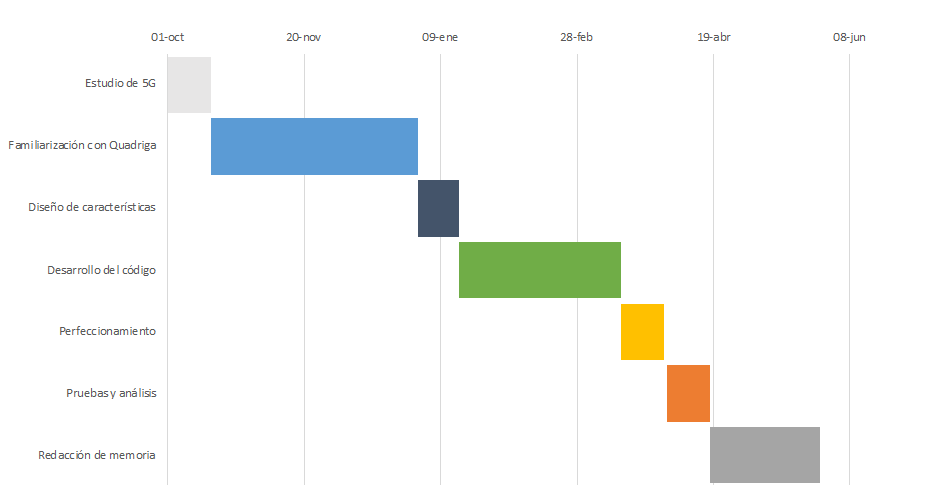
\includegraphics[width=\textwidth]{imagenes/gantt.PNG}
	\caption{Diagrama de Gantt de la distribución del trabajo a lo largo del curso 2017-18.}
	\label{fig:gantt}
\end{sidewaysfigure}

\clearpage

\section{Recursos y costes}

Aunque la realización de un \acs{tfg} no suele incurrir en gasto, no hay que dejar de tenerse en cuenta que el proyecto realizado se trata de un desempeño laboral que un profesional cualificado puede llevar a cabo aplicando los conocimientos que ha adquirido en el trascurso de su formación durante el grado. Por tanto, puede resultar conveniente realizar una estimación del gasto que el proyecto conllevaría en caso de realizarse en un marco laboral.

Para esta tarea, se ha hecho inventario del número de horas de trabajo por parte de cada una de las personas que han participado en el proyecto con su consecuente coste, así como de recursos físicos y lógicos que se han utilizado en el trascurso de desarrollo del proyecto.

\subsection{Recursos humanos}

Como se mencionaba en anteriores capítulos, la realización del proyecto ha sido principalmente llevada a cabo por el alumno \myName, que se puede considerar Graduado en \myDegree, con un coste por unidad horaria de 20,00 euros, junto a sus tutores \myProf, Profesor Ayudante Doctor, y \myOtherProf, Profesor Titular de Universidad, ambos doctores, cuyo coste por unidad horaria de trabajo se ha estimado en 60,00 euros.

Además, ha sido de gran ayuda la colaboración del investigador principal responsable del proyecto de desarrollo de \textit{QuaDRiGa}, Stephan Jaeckel, Ph.D., del \textit{Fraunhofer Heinrich-Hertz-Institut}, cuyo coste, del mismo modo, se ha estimado en 60,00 euros por unidad horaria.

En total, las reuniones de tutoría han acumulado 30 horas aproximadamente. Si a ese tiempo se le suman las horas de trabajo por parte de los tutores, de revisión, preparación de material y evaluación, el tiempo total asciende a 50 horas. Por otro lado, la ayuda prestada por parte del Doctor Jaeckel se estima en 5 horas.

Recopilando todas las horas de trabajo y realizando un desglose de las horas a sus respectivos costes, se puede hacer un cálculo estimado del coste del proyecto destinado a mano de obra, como se puede ver en la Tabla \ref{tab:sueldos}:

\begin{table}[h!]
\centering
\caption{Desglose de los costes de los participantes del proyecto}
\label{tab:sueldos}
\begin{tabular}{|m{5cm}|c|c|}
\hline
\textbf{Título / Puesto laboral}        & \multicolumn{1}{l|}{\textbf{Tiempo (h)}} & \multicolumn{1}{l|}{\textbf{Coste total (\euro)}} \\ \hline
Ingeniero Técnico de Telecomunicación & 380                                      & 9.500                                         \\ \hline
Profesor Ayudante Doctor                & 50                                       & 3.000                                         \\ \hline
Profesor Titular Doctor                 & 50                                       & 3.000                                         \\ \hline
Personal Investigador Doctor            & 5                                        & 300                                           \\ \hline
\multicolumn{2}{|c|}{\textbf{Coste total por mano de obra}}                        & \textbf{15.800}                               \\ \hline
\end{tabular}
\end{table}

Por tanto, el presupuesto total de recursos humanos para el proyecto asciende a la cantidad de quince mil ochocientos euros (15.800 \euro).

\subsection{Recursos software}

El proyecto se ha realizado utilizando un ordenador de uso personal que cuenta con el sistema operativo Windows, concretamente, Windows 10 Pro para equipos de 64 bits. Este sistema operativo es de pago y una licencia de uso indefinido está situada en un coste de 259,00 euros.

Por otro lado, la plataforma de desarrollo utilizada en este caso ha sido Matlab, versión R2017a, puesto que \textit{QuaDRiGa} está escrito para dicha plataforma. Este software tiene un coste de 2.000 euros para una licencia individual perpetua.

Para las fases de documentación, diseño y perfeccionamiento, se ha hecho uso de una suscripción a IEEExplore, una plataforma de base de datos de artículos y publicaciones de IEEE. Aunque la Universidad cuenta con su propia suscripción, una suscripción individual está valorada en 35 euros al mes, que durante ocho meses hacen un total de 280 euros.

También se ha hecho uso de otras herramientas gratuitas como correo electrónico para comunicaciones con los tutores y con el Dr. Jaeckel y el navegador de internet Mozilla Firefox para búsqueda primaria de información.

Por tanto, el proyecto debería destinar para recursos de software un total de dos mil quinientos treinta y nueve euros (2.539 \euro).

\subsection{Recursos hardware}

\begin{figure}[h!]
	\centering
    
\includegraphics[width=0.7\linewidth]{imagenes/ordenador.jpg}
	\caption{Imagen del ordenador utilizado.}
	\label{fig:ordenador}
\end{figure}

Para la realización de este proyecto no se necesita más que un ordenador de uso personal (PC). En concreto, el modelo utilizado es un Asus K55VD, que cuenta con las características técnicas reflejadas en la Tabla \ref{tab:caracteristicas}.

\begin{table}[h!]
\centering
\caption{Características técnicas del ordenador utilizado.}
\label{tab:caracteristicas}
\begin{tabular}{|c|c|}
\hline
Procesador     & Intel Core i7 3670QM                                                   \\ \hline
Memoria        & DDR3 1600 MHz 8 GB SDRAM                                               \\ \hline
Gráfica        & NVIDIA GeForce 610M con 2 GB  DDR3                                     \\ \hline
Almacenamiento & \begin{tabular}[c]{@{}c@{}}1 TB HDD 5400 RPM\\ 256 GB SSD\end{tabular} \\ \hline
\end{tabular}
\end{table}

Este equipo tiene un precio de venta al público de 729 euros y cuenta con la suficiente potencia como para ejecutar iteraciones del simulador en apenas unos minutos, como se muestra en el Capitulo 6.

\subsection{Coste total del proyecto}

Tras haber recopilado los detalles económicos de cada uno de los recursos involucrados en el proyecto, es posible realizar una estimación del coste total que supondría la realización del mismo en un ámbito profesional:

\begin{table}[h!]
\centering
\caption{Estimación del presupuesto total del proyecto.}
\label{tab:presupuesto}
\begin{tabular}{|c|c|}
\hline
\textbf{Recurso}     & \textbf{Coste (\euro)} \\ \hline
Personal             & 15.800                                \\ \hline
Software             & 2.539                                 \\ \hline
Hardware             & 729                                   \\ \hline
\textbf{Coste total} & \textbf{19.068}                       \\ \hline
\end{tabular}
\end{table}

Por tanto, este \acl{tfg} habría supuesto un coste total de diecinueve mil sesenta y ocho euros (19.068 \euro).